This layer is the integration of the UI and camera via Raspberry Pi as well as the mediator between the user and the UR5. The Node.js environment and OpenCV library are the main software involved in this layer.

\subsection{Control Layer Hardware}
N/A

\subsection{Control Layer Operating System}
N/A

\subsection{Control Layer Software Dependencies}
N/A

\subsection{Raspberry Pi}
The Raspberry Pi is a piece of hardware that establishes a virtual Node.js server to run the UI for the user interact with.  It also communicates with the Network Layer via Ethernet in order to issues commands to the UR5 due to user input.

\begin{figure}[h!]
	\centering
 	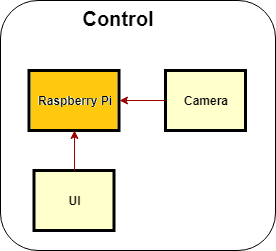
\includegraphics[width=0.60\textwidth]{images/Control_Layer_Raspberry_Pi}
 \caption{Raspberry Pi subsystem}
\end{figure}

\subsubsection{Raspberry Pi Subsystem Hardware}
Raspberry Pi 3 is the main hardware us in this subsystem. It has inputs for connecting the Ethernet cable to the Network Layer and USB and HDMI for connecting to the UI layer (mouse and monitor).

\subsubsection{Raspberry Pi Subsystem Operating System}
Debian GNU/Linux OS running on Raspberry Pi to initiate code.

\subsubsection{Raspberry Pi Subsystem Software Dependencies}
OpenCV and Node.js with NPM (Node Package Manager) to ensure all libraries are installed.

\subsubsection{Raspberry Pi Subsystem Programming Languages}
JavaScript, and HTML are used for establishing the Node.js server. Python 3.6 is used as a means of interpreting and sending URScript commands (Universal Robotics's internal robotic programming language) to the UR5. C++ is used handling camera interactivity with the OpenCV library (Not fully implemented).

\subsubsection{Raspberry Pi Subsystem Data Structures}
Structure of commands issued from Raspberry Pi to UR5 are sent as strings converted to bytes. For example the string 'stop(1.0)' would be converted to bytes and sent to the robot to tell it to stop.

\subsubsection{Raspberry Pi Subsystem Data Processing}
N/A

\subsection{Camera (Not fully implemented)}
The camera subsystem provide a video feed to the Raspberry Pi for image processing.

\begin{figure}[h!]
	\centering
 	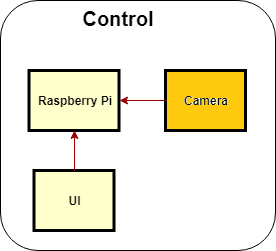
\includegraphics[width=0.60\textwidth]{images/Control_Layer_Camera}
 \caption{Camera subsystem}
\end{figure}

\subsubsection{Camera Subsystem Hardware}
The camera itself is a 720p web cam.

\subsubsection{Camera Subsystem Operating System}
N/A

\subsubsection{Camera Subsystem Software Dependencies}
N/A

\subsubsection{Camera Subsystem Programming Languages}
N/A

\subsubsection{Camera Subsystem Data Structures}
N/A

\subsubsection{Camera Subsystem Data Processing}
N/A

\subsection{User Interface (UI)}
The UI is the main interface the user uses to issues commands to the UR5 robotic arm.

\begin{figure}[h!]
	\centering
 	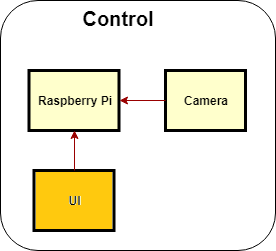
\includegraphics[width=0.60\textwidth]{images/Control_Layer_UI}
 \caption{UI subsystem}
\end{figure}

\subsubsection{UI Subsystem Hardware}
This subsystem uses a monitor and mouse connected to the Raspberry Pi and displays a UI with several buttons for the user to click in order to tell the UR5 what do.

\subsubsection{UI Subsystem Operating System}
N/A

\subsubsection{UI Subsystem Software Dependencies}
A virtual Node.js server with JavaScript as back-end of the UI is required.

\subsubsection{UI Subsystem Programming Languages}
JavaScript, and HTML are used for establishing the Node.js server. 

\subsubsection{UI Subsystem Data Structures}
N/A

\subsubsection{UI Subsystem Data Processing}
N/A
